%===============================================================================
\chapter{Identifica��o de sistemas n�o lineares utilizando refer�ncia virtual}
\label{chapter:dbnarmax}
%===============================================================================

Este cap�tulo tem o intuito de apresentar a ideia e os resultados obtidos da utiliza��o de refer�ncia virtual e
identifica��o de sistemas n�o lineares.  Na se��o \ref{sec:dbnarmax_nonlinear} introduz-se a id�ia de utiliza��o de
m�todos de projeto de controladores baseados em dados, juntamente com a utilzia��o de refer�ncia virtual para a obten��o
dos sinais necess�rios. Esta se��o utiliza o algoritmo apresentado na se��o \ref{sec:nl_si_algorithms_rationals} para
identifica��o de sistemas n�o lineares que podem ser descritos por classes de modelos NARMAX polinomiais ou racionais.
Alguns exemplos ser�o apresentados para que se possa avaliar a qualidade das estimativas obtidas.

%===============================================================================
%===============================================================================
\section{Introdu��o}
\label{sec:dbnarmax_intro}
%===============================================================================

Projeto de controladores descrito no Cap�tulo \ref{chapter:dbcd} tem como base a identifica��o de controladores
lineares. Encontram-se poucos trabalhos na literatura que abordam identifica��o de controladores n�o lineares baseados
nos dados coletados da planta. Em \cite{Guardabassi} � apresentado um procedimento para lineariza��o de sistemas n�o
lineares utilizando a ideia de refer�ncia virtual. Em \cite{campi_savaresi2006} � apresentada uma generaliza��o do
m�todo VRFT que envolve a identifica��o de controladores n�o lineares. Seguindo nesta linha, existem diversos trabalhos
propondo metodologias e algoritmos para a identifica��o de sistemas n�o lineares para in�meras fam�lias de modelos. Em
\cite{chen_billings1989Prediction} � apresentado uma metodologia para a estimativa de par�metros de sistemas n�o
lineares, de forma recursiva. Os mesmos autores no mesmo ano apresentaram um trabalho sobre identifica��o de sistemas
n�o lineares utilizando classes de modelos NARMAX \cite{chen_billings1989}. Em \cite{Hjalmarsson2012} � apresentada uma
modelagem de ordem finita de um modelo Hammerstein e sua acuracidade, modelagem esta que serve como refer�ncia para
parte do desenvolvimento que ser� apresentado na Se��o \ref{sec:dbnarmax_wiener_hammerstein}.

Existem na literatura diversos tipos de aplica��es para o conceito de refer�ncia virtual, para projeto de controladores
baseados em dados, o m�todo VRFT � talvez o mais conhecido. Neste trabalho tem-se o intuito de, baseado em refer�ncia
virtual, determinar os sinais de entrada para a utiliza��o de algum algoritmo de identifica��o de sistemas n�o
lineares, para com isso determinar qual � o controlador �timo para que o sistema se comporte em malha fechada como
desejado.


% ===============================================================================
\section{Exemplos ilustrativos}
\label{sec:dbnarmax_nonlinear_examples}
%===============================================================================

Neste trabalho o foco est� em apresentar os resultados da identifica��o de sistemas que podem ser descritos por modelos
NARMAX racionais ou polinomiais. Sendo que para isso ser�o apresentados exemplos de identifica��o de sistemas onde a
linearidade � est�tica assim como quando a n�o linearidade est� na din�mica do sistema.

Nos exemplos abordados a seguir as n�o linearidades estar�o presentes na planta do sistema e deseja-se que este sistema
se comporte em malha fechada como um sistema linear. Para isso o controlador adicionado na malha dever� ser capaz de
anular a n�o linearidade contida na planta, desta forma, for�ozamente o controlador ser� n�o linear, sendo descrito por
um modelo NARMAX racional ou polinomial.

Os exemplos apresentados a seguir s�o divididos em duas categorias: uma delas onde a n�o linearidade da planta est�
acoplada de forma est�tica e outra quando a n�o linearidade est� na din�mica do processo.

%===============================================================================
\subsection{N�o linearidades est�ticas}
\label{sec:dbnarmax_nl_wiener}
%===============================================================================

A planta do sistema utilizada neste exemplo possui uma n�o linearidade est�tica do tipo Wiener, onde o bloco n�o linear
encontra-se na sa�da do processo. Na Figura \ref{fig:vrft_nl_wiener} � apresentado o diagrama de blocos do sistema,
sendo $\zeta(t)$ e $\gamma(t)$ os blocos n�o lineares da planta e do controlador respectivamente. An�logamente
$G'(z)$ e $C'(z)$ s�o os blocos lineares da planta e do controlador. Como a n�o linearidade do controlador est� na
entrda deste, pode ser caracterizado como uma classe de Hammerstein, mas ser� identificado por uma classe de modelos
NARMAX racional.

\begin{figure}[htbp]
\center
% Generated with LaTeXDraw 2.0.8
% Sat Jun 16 14:47:44 BRT 2012
% \usepackage[usenames,dvipsnames]{pstricks}
% \usepackage{epsfig}
% \usepackage{pst-grad} % For gradients
% \usepackage{pst-plot} % For axes
\scalebox{1} % Change this value to rescale the drawing.
{
\begin{pspicture}(0,-1.72)(13.22,1.7)
\psline[linewidth=0.04cm,arrowsize=0.05291667cm 2.0,arrowlength=1.4,arrowinset=0.4]{->}(0.0,0.7)(1.0,0.7)
\pscircle[linewidth=0.04,dimen=outer](1.2,0.7){0.2}
\psline[linewidth=0.04cm,arrowsize=0.05291667cm 2.0,arrowlength=1.4,arrowinset=0.4]{->}(1.4,0.7)(2.8,0.7)
\psframe[linewidth=0.04,dimen=outer](4.0,1.1)(2.8,0.3)
\psline[linewidth=0.04cm,arrowsize=0.05291667cm 2.0,arrowlength=1.4,arrowinset=0.4]{->}(4.0,0.7)(5.0,0.7)
\psframe[linewidth=0.04,dimen=outer](6.2,1.1)(5.0,0.3)
\psframe[linewidth=0.04,dimen=outer](9.2,1.1)(8.0,0.3)
\psline[linewidth=0.04cm,arrowsize=0.05291667cm 2.0,arrowlength=1.4,arrowinset=0.4]{->}(9.2,0.7)(10.2,0.7)
\psframe[linewidth=0.04,dimen=outer](11.4,1.1)(10.2,0.3)
\psline[linewidth=0.04cm,arrowsize=0.05291667cm 2.0,arrowlength=1.4,arrowinset=0.4]{->}(6.2,0.7)(8.0,0.7)
\psline[linewidth=0.04cm,arrowsize=0.05291667cm 2.0,arrowlength=1.4,arrowinset=0.4]{->}(11.4,0.7)(13.2,0.7)
\psline[linewidth=0.04cm,arrowsize=0.05291667cm 2.0,arrowlength=1.4,arrowinset=0.4]{<-}(1.2,0.5)(1.2,-1.7)
\psline[linewidth=0.04cm](1.2,-1.7)(12.4,-1.7)
\psline[linewidth=0.04cm](12.4,-1.7)(12.4,0.7)
\usefont{T1}{ppl}{m}{n}
\rput(0.45828125,1.01){$r(t)$}
\usefont{T1}{ppl}{m}{n}
\rput(1.9445312,1.01){$\epsilon (t)$}
\usefont{T1}{ppl}{m}{n}
\rput(4.514531,1.01){$v(t)$}
\usefont{T1}{ppl}{m}{n}
\rput(7.089375,1.01){$u(t)$}
\usefont{T1}{ppl}{m}{n}
\rput(9.664532,1.01){$\omega(t)$}
\usefont{T1}{ppl}{m}{n}
\rput(12.499375,1.01){$y(t)$}
\psline[linewidth=0.04cm](1.6,0.5)(1.8,0.5)
\psframe[linewidth=0.04,linestyle=dashed,dash=0.16cm 0.16cm,dimen=outer](6.6,1.7)(2.4,-0.3)
\psframe[linewidth=0.04,linestyle=dashed,dash=0.16cm 0.16cm,dimen=outer](11.8,1.7)(7.6,-0.3)
\usefont{T1}{ppl}{m}{n}
\rput(4.3345313,-0.59){C(z)}
\usefont{T1}{ppl}{m}{n}
\rput(9.744532,-0.59){G(z)}
\usefont{T1}{ppl}{m}{n}
\rput(3.3945312,0.69){$\gamma(t)$}
\usefont{T1}{ppl}{m}{n}
\rput(10.794531,0.71){$\zeta(t)$}
\usefont{T1}{ppl}{m}{n}
\rput(5.594531,0.71){C'(z)}
\usefont{T1}{ppl}{m}{n}
\rput(8.604531,0.71){G'(z)}
\end{pspicture} 
}

\caption{Diagrama de blocos para um sistema n�o linear do tipo Wiener}
\label{fig:vrft_nl_wiener}
\end{figure}

O sistema possui um boloco linear que pode ser descrito por:

\begin{equation}
G'(z)=\frac{0.5}{z-0.9}
\label{eq:vrft_nl_wiener_g}
\end{equation} 

O comportamento do sistema em malha fechada esperado � definido por $M(z)$:

\begin{equation}
M(z)=\frac{0.4}{z-0.6}
\label{eq:vrft_nl_wiener_m}
\end{equation}  

A n�o linearidade presente na planta do sistema foi escolhida como sendo um polin�mio de terceira ordem
descrito como abaixo:

\begin{equation}
\zeta(\omega(t))=y(t)=1.5\omega(t)+0.2\omega^3(t)
\label{eq:vrft_nl_wiener_phi}
\end{equation}  

Espera-se ent�o que por $M(z)$ ser linear, que o controlador tenha um bloco que cancele o efeito n�o linear de
$\zeta(t)$.

Deseja-se que em malha fechada o sinal $v(t)$ seja tal que:

\begin{equation}
v(t)=r(t)-\omega(t)
\end{equation}

Tem-se entretanto:

\begin{equation}
v(t)=\epsilon(t)\gamma (t)
\nonumber
\end{equation}

e que

\begin{equation}
\epsilon(t) = r(t) - y(t)
\nonumber
\end{equation}
 
Obtem-se ent�o o relacionamento entre os sinais $\gamma (t) $ e $\zeta(t)$:

\begin{equation}
( r(t) - \omega(t) \zeta(t)) \gamma (t) = r(t) - \omega(t) 
\nonumber
\end{equation}

Resultando:

\begin{equation}
\gamma (t) = \frac{r(t)-\omega(t)}{r(t) - \omega(t)\zeta(t)} 
\end{equation}

Pecebe-se claramente que quando n�o h� sinal de refer�ncia $r(t)$, o relacionamento entre os polinomios $\gamma (t) $
e $\zeta(t)$ fica simplificado a:

\begin{equation}
\gamma (t) = \frac{1}{\zeta(t)}
\nonumber 
\end{equation}

Define-se ent�o $\gamma (t)$ como sendo:

\begin{equation}
\gamma (\epsilon(t))= v(t) = a_1\epsilon (t) + a_2 \epsilon ^2(t) +a_3 \epsilon ^3(t) +a_4 \epsilon ^4(t)
\label{eq:vrft_nl_wiener_phi_inv}
\end{equation}  

Desconsiderando a parte n�o linear presente na planta, � simples de observar que o controlador �timo que
levaria a planta em malha fechada a ter o comportamento descrito por $M(z)$ �:

\begin{equation}
C_d(z)= \frac{0.8z-0.72}{z-1}
\label{eq:vrft_nl_wiener_cd}
\end{equation}  

O controlador $C_d(z)$ possui uma integrador em sua estrutura. Para evitar problemas de seguimento de
refer�ncia optou-se por n�o identificar esta parte do controlador. Mantendo o denominador como um integrador
e identificando apenas o numerador. Juntamente com a identifica��o do controlador da por��o linear $C_d(z)$ �
necess�rio identificar o polin�mio da equa��o \eqref{eq:vrft_nl_wiener_phi_inv}.

Fazendo-se as substitui��es matem�ticas necess�rias, chega-se a express�o do sinal de sa�da do controlador que
se quer identificar:

\begin{equation}
u(t)=\begin{bmatrix}
\theta_1 & \theta_2 & \theta_3 & \theta_4 & \theta_5 & \theta_6 & \theta_7 & \theta_8
\end{bmatrix}
\begin{bmatrix}
\epsilon (t)\\ 
\epsilon ^2(t)\\ 
\epsilon^3(t)\\ 
\epsilon^4(t)\\ 
\epsilon(t-1)\\ 
\epsilon^2(t-1)\\ 
\epsilon^3(t-1)\\ 
\epsilon^4(t-1)
\end{bmatrix}
\label{eq:vrft_nl_wiener_u}
\end{equation}  

Onserva-se que $u(t)$ em \eqref{eq:vrft_nl_wiener_u} � um modelo NARMAX polinomial. Foram realizados 100 experimentos
de Monte Carlo utilizando o algoritmo para identifica��o de modelos NARMAX em conjunto com o procedimento de refer�ncia
virtual para gerar os sinais $r(t)$ e $\epsilon(t)$ e a m�dia das estimativas obtidas foi de:

\begin{equation}
\text{m�dia }\;\theta =\begin{bmatrix}
0.4471 \\ 0.0020 \\ -6.5105\times10^{-4} \\ -1.5959\times10^{-5} \\ -0.4043 \\ -0.0016 \\ 6.1194\times10^{-4}
\\ 1.4562\times10^{-5}
\end{bmatrix}^T
\nonumber
\end{equation}

Com um desvio padr�o de:

\begin{equation}
\text{m�dia }\;\theta = 1\times10^{-3}\begin{bmatrix}
0.2430 \\ 0.0246 \\ 0.0015 \\ 0.0001 \\ 0.2613 \\ 0.0259 \\ 0.0016 \\ 0.0001
\end{bmatrix}^T
\nonumber
\end{equation}

O custo entre os sinais de sa�da do sistema obtido e o sistema esperado $M(z)$ foi de  $J_{MR}(\theta)=
0.3820$ e o custo dos sinais de sa�da do controlador ($u(t)$) esperado e obtido foi de $J_{VR}=1.0119$.

Como a estimativa de $\gamma (\epsilon(t))$ � apenas uma aproxima��o do que espera-se ser a inversa de
$\zeta(\omega(t))$, a classe de modelos escolhida para o controlador n�o consegue representar a totalidade do
controlador ideal. Desta forma � esperado que a identifica��o n�o consiga atingir a totalidade da fun��o
$M(z)$ inicialmente escolhida. Para as estimativas foram utilizados sinais de entrada do tipo PRBS com 127 pontos para a
excita��o da planta.

Na Figura (\ref{fig:vrft_nl_wiener_step}) � apresentado um comparativo entre o sinal de sa�da do sistema
$M(z)$ quando submetido a um degrau unit�rio e o sinal do sistema real quando o controlador identificado �
aplicado sobre a planta em malha fechada.

\begin{figure}[htbp] 
	\center 
	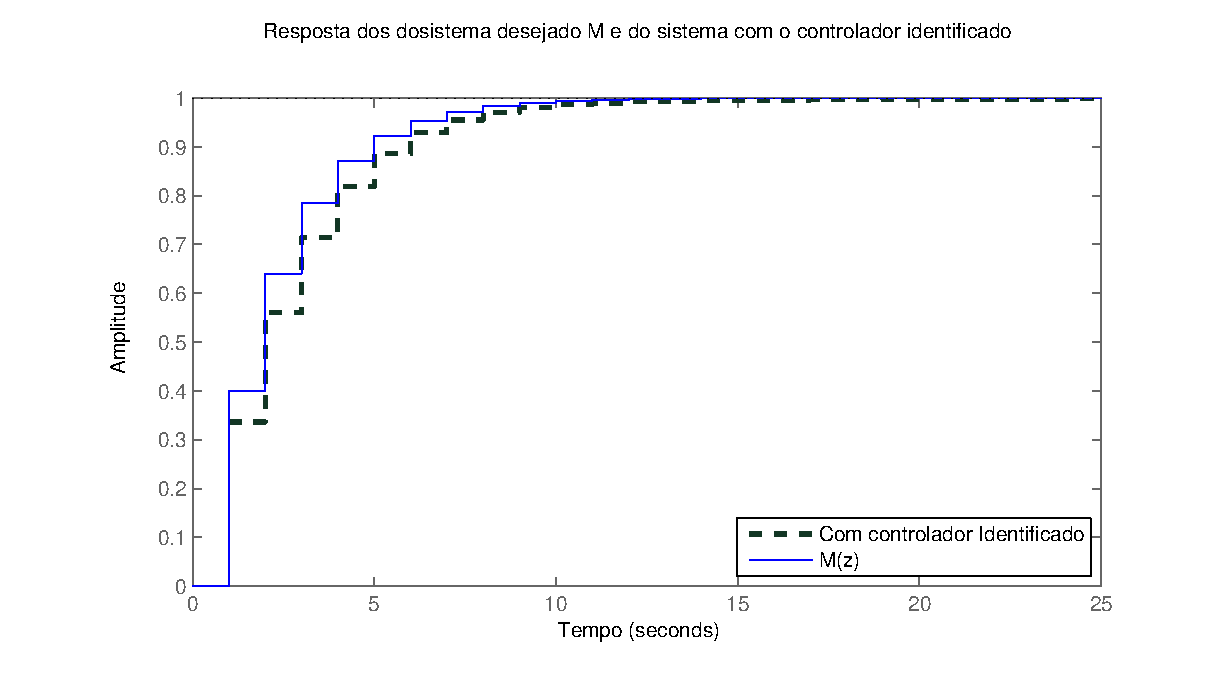
\includegraphics[width=0.95\columnwidth]{figures/vrft_nl_wiener_step.eps}
	\caption{resposta dos sistemas: desejado e obtido a um degrau unit�rio}
	\label{fig:vrft_nl_wiener_step}
\end{figure}

Na Figura (\ref{fig:vrft_nl_wiener_vw_step}) � apresentado o comportamento dos sinais de sa�da e entrada das
n�o linearidades $\gamma(\epsilon(t))$ e $\zeta(\omega(t))$ respectivamente.

\begin{figure}[htbp] 
	\center 
	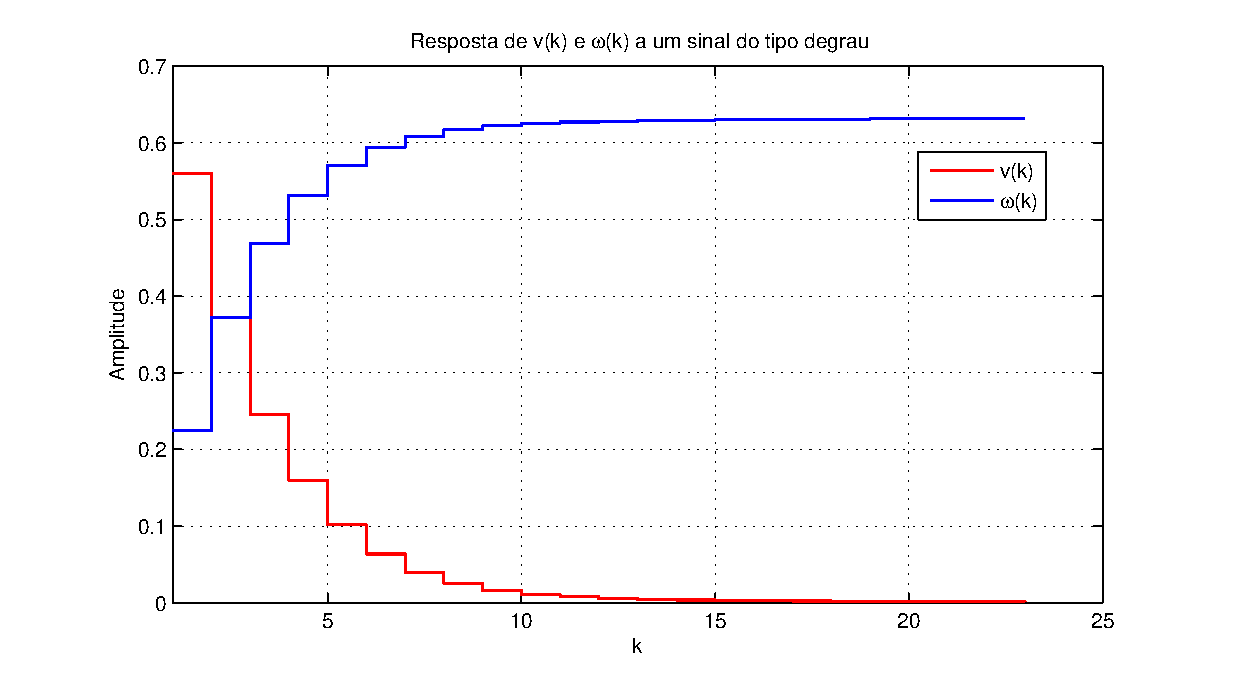
\includegraphics[width=0.95\columnwidth]{figures/vrft_nl_wiener_vw_step.eps}
	\caption{sinais $v(t)$ e $\omega(t)$ quando o sistema � alimentado por um degrau unit�rio}
	\label{fig:vrft_nl_wiener_vw_step}
\end{figure}

A rela��o entre os sinais $v(t)$ e $\omega(t)$ � apresentado na Figura (\ref{fig:vrft_nl_wiener_vw}).
Observa-se que a rela��o destes sinais � praticamente linear, garantido que a aproxima��o de $\gamma(\epsilon(t))$
foi satisfat�ria para representar a inversa do sinal $\zeta(\omega(t))$.

\begin{figure}[htbp] 
	\center 
	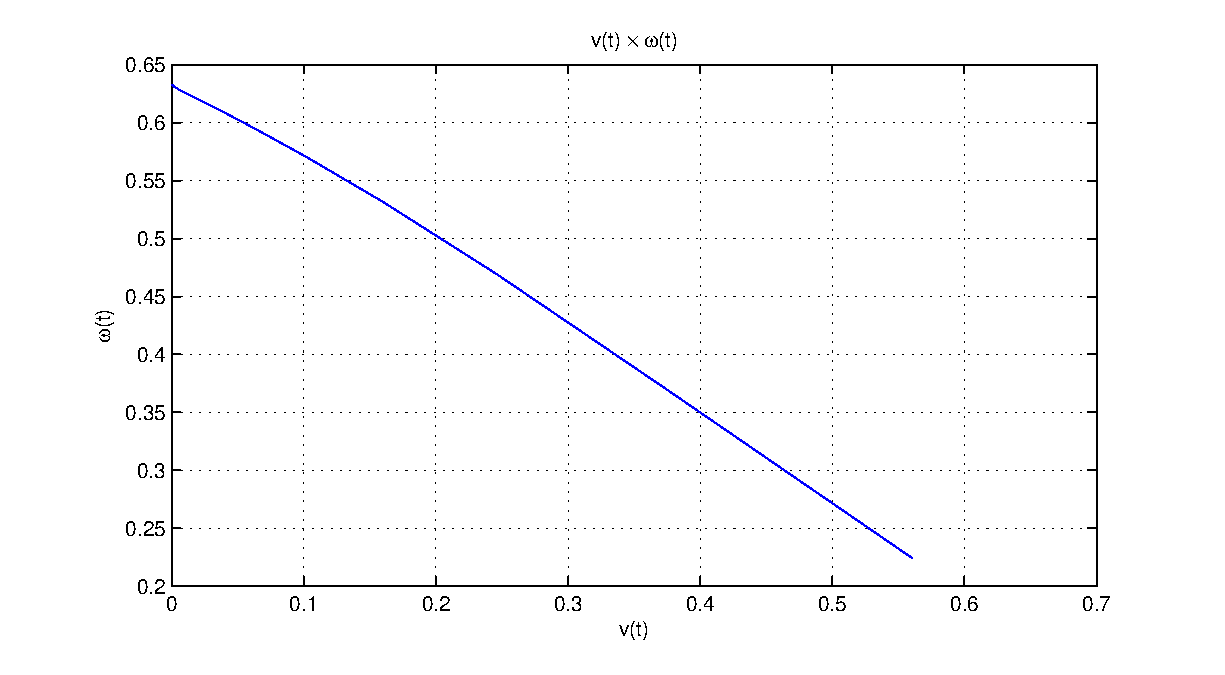
\includegraphics[width=0.95\columnwidth]{figures/vrft_nl_wiener_vw.eps}
	\caption{rela��o entre os sinais $v(t)$ e $\omega(t)$ quando o sistema � alimentado por um degrau unit�rio}
	\label{fig:vrft_nl_wiener_vw}
\end{figure}

%===============================================================================
\subsection{N�o linearidades din�micas}
\label{sec:dbnarmax_nl_dinamic}
%===============================================================================

Quando a n�o linearidade est� na din�mica do processo n�o h� uma distin��o entre um bloco linear e outro linear como
apresentado no exeplo anterior (se��o \ref{sec:dbnarmax_nl_wiener}). Ser�o apresentados aqui alguns exemplos de
identifica��o de controladores que podem ser representados por modelos NARMAX racionais.

Inicialmente um exemplo onde o controlador que leva a planta $G_0(z)$ a se comportar em malha fechada como em $M(z)$,
ser� totalmente representado pelo modelo escolhido para o controlador. Em seguida ser� apresentado para esta mesma
situa��o onde o controlador necess�rio � um pouco mais complexo, tendo mais vari�veis para identificar.

Ao fim ser� apresentado um exemplo onde o controlador ideal n�o consegue ser representado pela classe de modelos
escolhida.

Em todos os exemplos ser� utilizado para excitar o sistema, um sinal PRBS de ordem 7.

%===============================================================================
\subsubsection{Controlador ideal sendo representado pela classe de modelos}
\label{sec:dbnarmax_nl_dinamic_c_match}
%===============================================================================

Neste exemplo ser� abordado o caso onde o controlador $C(z, \theta) \in \mathcal{C}$. Fazendo com que o sistema em
malha fechada se comporte como desejado. Considere a planta n�o linear descrita por:

\begin{equation}
y(t)=\frac{0.5u(t-1)y(t-1)+u(t-1)}{1+0.25y^2(t-2)}
\label{eq:vrft_nl_dinamic_ex1_y}
\end{equation}

Deseja-se que em malha fechada seu comportamento seja linear como em:

\begin{equation}
M(z)=\frac{0.4}{z-0.6}
\label{eq:vrft_nl_dinamic_ex1_mz}
\end{equation}

A equa��o \eqref{eq:vrft_nl_dinamic_ex1_mz} pode ser reescrita em fun��o do tempo como em:

\begin{equation}
y(t)=0.4r(t-1)+0.6y(t-1)
\label{eq:vrft_nl_dinamic_ex1_mt}
\end{equation}

Ao igualar a equa��o \eqref{eq:vrft_nl_dinamic_ex1_y} com \eqref{eq:vrft_nl_dinamic_ex1_mt} e isolar o
sinal $u(t)$ tem-se a equa��o que descreve o comportamento do controlador que levar� a planta a ter o
comportamento descrito por $M(z)$ em malha fechada. Obt�m-se desta forma um controlador ideal como em:

\begin{equation}
u(t)=\frac{0.4r(t)+0.6y(t)+0.1y^2(t-1)r(t)+0.15y(t)y^2(t-1)}{1+0.5y(t)}
\label{eq:vrft_nl_dinamic_ex1_cd}
\end{equation}

Escolhendo uma classe de modelos que consegue representar o controlador �timo:

\begin{equation}
u(t)=\frac{\theta_1 r(t)+ \theta_2 y(t)+ \theta_3 y^2(t-1)r(t)+ \theta_4 y(t)y^2(t-1)}{1+ \theta_5 y(t)}
\label{eq:vrft_nl_dinamic_ex1_c}
\end{equation}

Utilizando um sinal PRBS de tamanho 254 pontos e o m�todo de refer�ncia virtual para gerar os sinais $r(t)$ e
$\epsilon(t)$. Adicionando-se um ruido de vari�ncia $\sigma^2 = 0.005$ a sa�da do sistema, a m�dia das estimativas para
100 experimentos de Monte Carlo foi de:

\begin{equation}
\theta_{\text{m�dia}}=\begin{bmatrix}
0.4000 & 0.5999 & 0.1001 & 0.1501 & 0.5000
\end{bmatrix}
\nonumber
\end{equation}

Os valores reais utilizados na simula��o foram:

\begin{equation}
\theta_0=\begin{bmatrix}
0.4 & 0.6 & 0.1 & 0.15 & 0.5
\end{bmatrix}
\nonumber
\end{equation} 

Obte-se um desvio padr�o para as estimativas de:

\begin{equation}
\theta_{\text{desvio padr�o}}=1.0\times 10^{-3}\begin{bmatrix}
0.2231 & 0.6866 & 0.2411 & 0.6817 & 0.3019
\end{bmatrix}
\nonumber
\end{equation}

A matriz de covari�ncia � descrita por:

\begin{equation}
\theta_{\text{Covari�ncia}}=1.0\times 10^{-6}\begin{bmatrix}
 0.0498 &  0.0585 & -0.0353 & -0.0362 & -0.0018 \\
 0.0585 &  0.4714 & -0.0449 & -0.3690 &  0.0057 \\
-0.0353 & -0.0449 &  0.0581 &  0.0745 & -0.0040 \\
-0.0362 & -0.3690 &  0.0745 &  0.4647 & -0.0070 \\
-0.0018 &  0.0057 & -0.0040 & -0.0070 &  0.0911
\end{bmatrix}
\nonumber
\end{equation}

Simulando o sistema com o controlador obtido pela m�dia das estimativas e o sistema em malha fechada
desejado, o erro observado para um sinal de entrada do tipo degrau unit�rio � apresentado na Figura
\ref{fig:vrft_nl_dynamic_step_erro}.

\begin{figure}[htbp] 
	\center 
	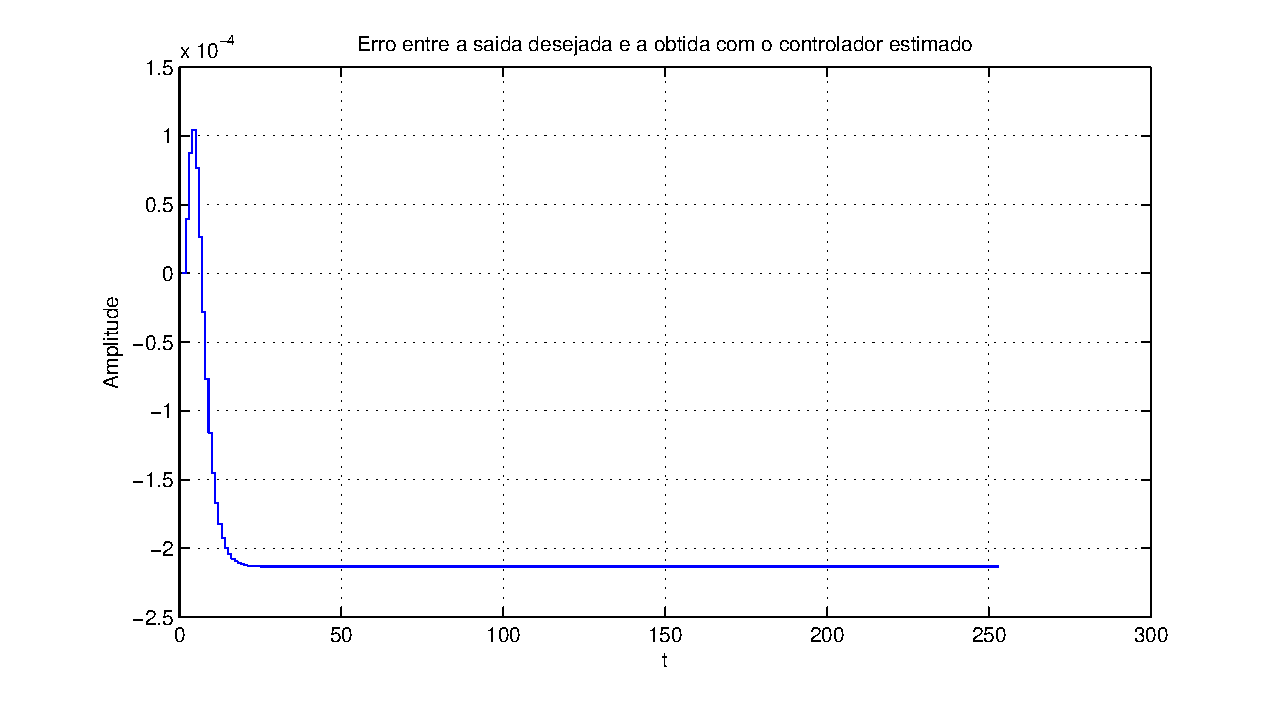
\includegraphics[width=0.95\columnwidth]{figures/vrft_nl_dynamic_erro_step.eps}
	\caption{Erro entre o a resposta esperada e obtida para uma entrada do tipo degrau unit�rio}
	\label{fig:vrft_nl_dynamic_step_erro}
\end{figure}

A fim de ilustrar as estimativas obtidas pelo m�todo, na Figura \ref{fig:vrft_nl_dynamic_t1_t2} s�o
apresentados as estimativas para os 100 experimentos realizados, al�m da elipse de confian�a de $\chi^2=95\%$
para os parametros $\theta_1$ e $\theta_2$.

\begin{figure}[htbp] 
	\center 
	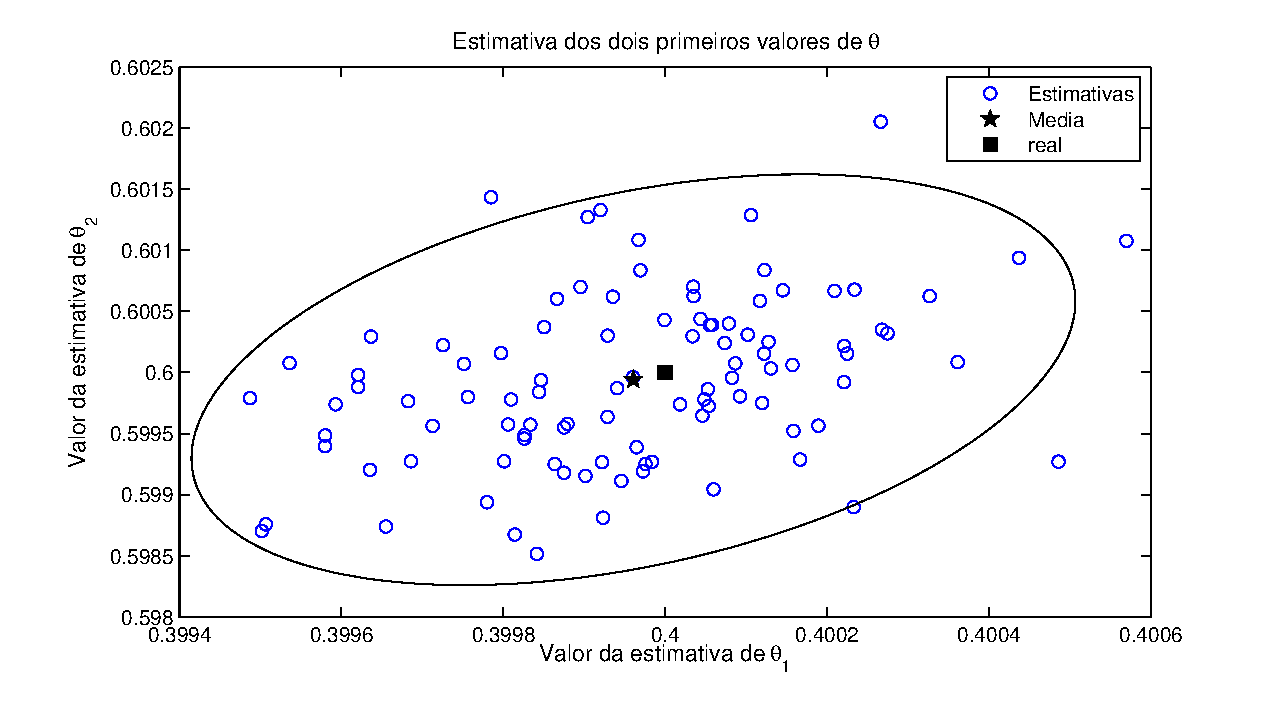
\includegraphics[width=0.95\columnwidth]{figures/vrft_nl_dynamic_t1_t2.eps}
	\caption{100 esperimentos de Monte Carlo das vari�veis $\theta_1$ e $\theta_2$}
	\label{fig:vrft_nl_dynamic_t1_t2}
\end{figure}

O custo $J_{VR}=2.7291\times10{-8}$ foi obtido utilizando-se os sinais de sa�da do controlador obtido e
esperado. J� o custo entre os sinais de sa�da do sistema em malha fechada estimado e desejado foi de
$J_{MR}=0.0033$.

Com o intuito de demonstrar o efeito do ru�do sobre as estimativas obtidas o ruido foi aumentado em $4\times$ para
$\sigma^2 = 0.02$. Obteve-se desta forma os seguintes resultados paras as estimativas:

\begin{equation}
\theta_{\text{m�dia}}=\begin{bmatrix}
0.3999 & 0.5996 & 0.1001 & 0.1502 & 0.4999
\end{bmatrix}
\nonumber
\end{equation}

\begin{equation}
\theta_{\text{Desvio padr�o}}=\begin{bmatrix}
0.0010 & 0.0027 & 0.0012 & 0.0027 & 0.0012
\end{bmatrix}
\nonumber
\end{equation}

\begin{equation}
\theta_{\text{Covari�ncia}}=1.0\times 10^{-5}\begin{bmatrix}
    0.1061 &  0.1207 & -0.0894 & -0.1185 & -0.0310 \\
    0.1207 &  0.7122 & -0.1048 & -0.5357 &  0.0038 \\
   -0.0894 & -0.1048 &  0.1344 &  0.1972 & -0.0033 \\
   -0.1185 & -0.5357 &  0.1972 &  0.7523 & -0.0571 \\ 
   -0.0310 &  0.0038 & -0.0033 & -0.0571 &  0.1355
\end{bmatrix}
\nonumber
\end{equation}

Com os custos de $J_{VR}=1.0326\times10{-7}$ e $J_{MR}=0.0054$, corroborando para o fato de que os custos n�o
foram significativamente afetados pelo aumento do ru�do. Fazendo assim com que a estimativa ainda seja confi�vel.

%===============================================================================
\subsubsection{Controlador ideal sendo representado pela classe de modelos 2}
\label{sec:dbnarmax_nl_dinamic_c_match2}
%===============================================================================

%===============================================================================
\subsubsection{Controlador n�o sendo representado pelo modelo}
\label{sec:dbnarmax_nl_dinamic_c_not_match}
%===============================================================================

Neste exemplo ser� abordado o caso onde o controlador $C(z, \theta) \notin \mathcal{C}$. Fazendo com que o sistema em
malha fechada n�o consiga ter a din�mica esperada. Considere a planta n�o linear descrita por:

\begin{equation}
y(t)=\frac{0.5u(t-1)y(t-1)+u(t-1)}{1+0.25y^2(t-2)}
\label{eq:vrft_nl_dinamic_ex3_y}
\end{equation}

Deseja-se que em malha fechada seu comportamento seja linear como em:

\begin{equation}
M(z)=\frac{0.4}{z-0.6}
\label{eq:vrft_nl_dinamic_ex3_mz}
\end{equation}

A equa��o \eqref{eq:vrft_nl_dinamic_ex3_mz} pode ser reescrita em fun��o do tempo como em:

\begin{equation}
y(t)=0.4r(t-1)+0.6y(t-1)
\label{eq:vrft_nl_dinamic_ex3_mt}
\end{equation}

Ao igualar a equa��o \eqref{eq:vrft_nl_dinamic_ex3_y} com \eqref{eq:vrft_nl_dinamic_ex3_mt} e isolar o
sinal $u(t)$ tem-se a equa��o que descreve o comportamento do controlador que levar� a planta a ter o
comportamento descrito por $M(z)$ em malha fechada. Obt�m-se desta forma um controlador ideal como em:

\begin{equation}
u(t)=\frac{0.4r(t)+0.6y(t)+0.1y^2(t-1)r(t)+0.15y(t)y^2(t-1)}{1+0.5y(t)}
\label{eq:vrft_nl_dinamic_ex3_cd}
\end{equation}

No exemplo apresentado na se��o \ref{sec:dbnarmax_nl_dinamic_c_match} foi apresentada a simula��o para quando o controlador
�timo consegue ser descrito pelo modelo escolhido para representa-lo. Neste exeplo deseja-se o oposto: que a classe de
modelos escolhida para o controlador n�o consiga representar completamente \eqref{eq:vrft_nl_dinamic_ex3_cd}. Para isso
escolheu-se a seguinte classe de modelos para representar o controlador:

\begin{equation}
u(t)=\frac{\theta_1 r(t)+ \theta_2 y(t)+ \theta_3 r(t)y(t-1)+ \theta_4 y(t-1)y(t)}{1+ \theta_5 y(t)}
\label{eq:vrft_nl_dinamic_ex3_c}
\end{equation}

Para as simula��es foi adicionado um ru�do com $\sigma^2 = 0.05$. Foram realizados 100 experimentos de Monte Carlo onde
obteve-se as seguintes estimativas:

\begin{equation}
\theta_{\text{m�dia}}=\begin{bmatrix}
0.4696 & 0.7011 & 0.0083 & 0.0063 & 0.5013
\end{bmatrix}
\label{eq:vr_rational_ex3_theta}
\end{equation}

\begin{equation}
\theta_{\text{Desvio padr�o}}=\begin{bmatrix}
0.0017 & 0.0058 & 0.0020 & 0.0064 & 0.0025
\end{bmatrix}
\nonumber
\end{equation}

\begin{equation}
\theta_{\text{Covari�ncia}}=1.0\times 10^{-4}\begin{bmatrix}
    0.0278 &  0.0396 &  0.0035 &  0.0146 & -0.0137 \\
    0.0396 &  0.3328 &  0.0066 & -0.1651 &  0.0063 \\
    0.0035 &  0.0066 &  0.0382 &  0.0688 & -0.0119 \\
    0.0146 & -0.1651 &  0.0688 &  0.4130 & -0.0562 \\
   -0.0137 &  0.0063 & -0.0119 & -0.0562 &  0.0646
\end{bmatrix}
\nonumber
\end{equation}

Obte-se um custo para o comportamento do sistema em malha fechada de  $J_{MR}=1.0999$. Na Figura
\ref{fig:vr_rational_notinclass_ex3_error} � apresentado o erro para o sistema desejado e o sistema obtido utilizando-se
o modelo obtido com os valores de $\theta$ apresentados em \eqref{eq:vr_rational_ex3_theta} para uma refer�ncia do tipo
degrau unit�rio.

\begin{figure}[htbp] 
	\center 
	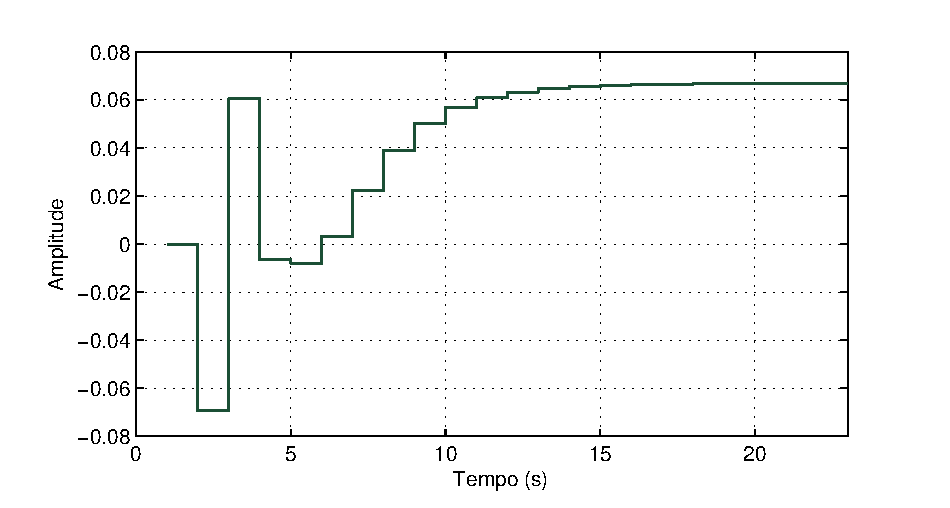
\includegraphics[width=0.95\columnwidth]{figures/vr_rational_notinclass_ex3_error.eps}
	\caption{Erro entre o comportamento do sistema em malha fechada e o comportamento em malha fechada desejado.}
	\label{fig:vr_rational_notinclass_ex3_error}
\end{figure}























%===============================================================================
\section{Considera��es Finais}
\label{sec:dbnarmax_conclusions}
%===============================================================================

Neste cap�tulo apresentou-se a uni�o das ideias de utiliza��o de refer�ncia virtual para a obten��o dos sinais
necess�rios para a determina��o do controlador �timo e a ideia de utiliza��o de algoritmos de identifica��o de sistemas
n�o lineares para determina��o do controlador �timo quando este faz parte de uma classe de modelos n�o linear.

Descreveu-se inicialmente a ideia generalizada onde a classe de modelos n�o linear do controlador precisa estar atrelada
apenas ao algoritmo utilizado para sua identifica��o. Devido aos bons resultados obtidos com a identifica��o de sistemas
NARMAX apresentados no Cap�tulo \ref{chapter:nlin_si_ident}, optou-se por utilizar este algoritmo (Se��o
\ref{sec:nl_si_algorithms_rationals}) para determinar os par�metros do controlador utilizando-se para isso entretanto
dos sinais obtidos por meio do m�todo de refer�ncia virtual.

Nas Se��es \ref{sec:dbnarmax_wiener_hammerstein} e \ref{sec:dbnarmax_rational_controllers} apresentou-se alguns
exemplos para demonstrar a viabilidade da utiliza��o da metodologia. Foram apresentados exemplos onde a classe de
modelos consegue representar a totalidade das din�micas de $\mathcal{C}_d$ para que o sistema se comporte em malha
fechada linearmente como escolhido por $T_d(z)$. Outro exemplo foi apresentado quando n�o existe uma completa descri��o
do controlador ideal pela classe de modelos, ou seja, $\mathcal{C}_d \notin \mathcal{C}$, apresentou-se um comparativo
do sistema ideal e do obtido utilizando o controlador obtido quando o sistema � submetido a um degrau unit�rio.

Tamb�m foi apresentado um exemplo onde o controlador � descrito por um modelo NARMAX polinomial, em um contexto onde a
planta do sistema possui uma n�o linearidade est�tica na sa�da do processo, caso este onde o controlador ideal tamb�m
n�o se encontra na classe de modelos. A aproxima��o do modelo escolhido para este controlador se mostrou relativamente
pr�ximo ao controlador ideal, visto que o cancelamento da n�o linearidade da planta foi quase completo, como apresentado
na Figura \ref{fig:vrft_nl_wiener_vw}.

De forma geral, apresentou-se neste cap�tulo a utiliza��o desta metodologia de identifica��o de controladores n�o
lineares descritos por modelos NARMAX, polinomial ou racional e seus resultados. Os resultados obtidos mostram que a
metodologia � v�lida e que em situa��es onde o controlador ideal pode ser bem representado pela classe de controladores,
os resultados obtidos n�o possuem erro de polariza��o para experimentos executados em malha aberta. 

%===============================================================================
